Der Miller-Rabin-Test ist ein probalistischer Primzahltest, dies bedeutet, dass der Algorithmus nicht immer zweifelsfrei korrekte Ergebnisse berechnet, jedoch kann die Genauigkeit der Ergenisse durch mehrfaches Durchlaufen des Algorithmus verbessert werden.
Der Miller-Rabin-Test hat für eine Iteration eine Wahrscheinlichtkeit kleiner als $\frac{1}{4}$ eine zusammengesetze Zahl als Primzahl zu erkennen. Aufgrund dessen ist es empfehlenswert den Algorithmus über mehrere Iterationen auszuführee, sodass die Wahrscheinlichtkeit des Fehlers vernachlässigbar wird.
Nach $i$ Iterationen ist die Wahrscheinlichtkeit des Fehlers $(\frac{1}{4})^i$. Somit ist sie für $10$ Iterationen schon rund $0.00000095367431640625$, was für die Primzahlselektion des RSA-Algorithmus ausreichend ist. Abbildung \ref{mr_error} zeigt den Verlauf der Fehlerwahrscheinlichkeit von $1$ bis $100$ Iterationen und illustriert deutlich, dass der Miller-Rabin-Test mit wenigen Iterationen einen ausreichend präziser Primzahltest bietet.

\begin{figure}[ht]
  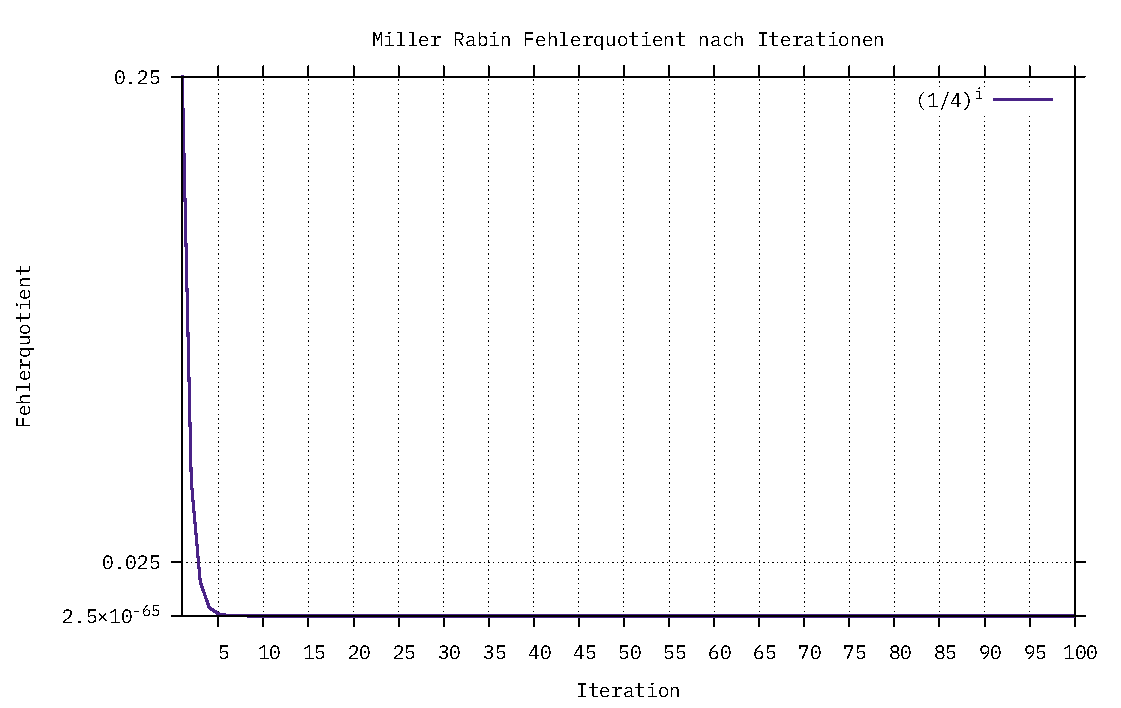
\includegraphics{mr_error.pdf}
  \label{mr_error}
  \caption{Fehlerquotient für $\left\{\,i \in \mathbb{N}\mid 1 \le i \le 100 \, \right\}$}
\end{figure}
